\chapter{The solver ecosystem}
\label{ch:c4}
\begin{keybox}
\textbf{Key idea.} Every implicit step ends in a linear solve of the
\emph{indefinite} $(c,\mu)$ Cahn--Hilliard saddle, and there is no single
best solver. Choose by measuring \emph{both} correctness (the residual)
and speed: a fast solver that returns a wrong answer is not fast. In 2-D,
correctness is not the deciding factor --- every backend is accurate ---
so speed decides; in 3-D the deciding factor is \emph{memory}, not
accuracy, and that is where the block preconditioner and matrix-free
methods take over.
\end{keybox}

This concept teaches how to choose, using a small live 2-D comparison ---
with the residual reported beside the speed --- plus the measured 3-D
scaling tables from the device-assembly and \texttt{blockch} development
notes.

\section{Correctness first, then speed}

Each Newton iterate solves $A\,\delta = r$, where $A$ is the mixed
$(c,\mu)$ Cahn--Hilliard Jacobian --- a \emph{saddle}-structured,
\emph{indefinite} sparse matrix. Indefiniteness is a real hazard: a
general-purpose GPU direct solver factorizes without the pivoting an
indefinite system may need, so \emph{in principle} it could return a
large-residual (wrong) answer. The scientific response is not to assume,
but to \textbf{verify}: solve the same captured system with each backend
and report the relative residual $\|A\delta-r\|/\|r\|$.

\begin{keybox}
\textbf{Measured (2-D, $\CfourCorrectDofs$ dofs).} Every backend is
accurate: \code{splu} (pivoted CPU direct) $\CfourSpluResid$, \textbf{cuDSS}
(GPU direct) $\CfourCudssResid$, and \texttt{blockch} (the CH-specific
block preconditioner) $\CfourBlockchResid$. The verification \emph{passes}
for each --- including cuDSS, which handles the indefinite 2-D saddle fine.
So in 2-D correctness does not pick the solver; \emph{speed} does. (This
overturns a tempting but unverified claim that cuDSS ``diverges on the CH
saddle''; on the systems measured here it does not. Always check the
residual rather than repeat folklore.)
\end{keybox}

\begin{figure}[h]\centering
  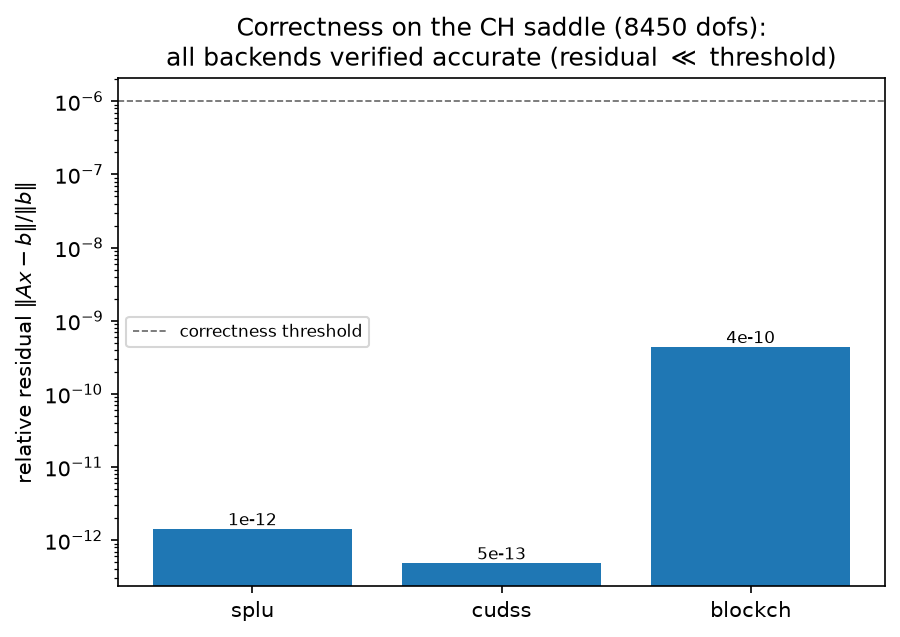
\includegraphics[width=0.6\linewidth]{figures/c4_correctness.png}
  \caption{Relative residual of each backend on the same captured CH
    saddle. All sit far below the correctness threshold ($10^{-6}$):
    \code{splu}, cuDSS, and \texttt{blockch} each solve the indefinite
    2-D saddle accurately. Correctness is proved, not assumed.}
  \label{fig:c4correct}
\end{figure}

\section{The 2-D crossover, measured live}

With correctness settled, speed decides in 2-D. We assemble the
\emph{real} Cahn--Hilliard Jacobian at three mesh sizes and time the
linear solve (factorize $+$ solve), cold and warm, CUDA-synchronised, as a
median. The full step is host-assembly-bound in this brick, which would
swamp the solver signal, so we isolate the solve.

\begin{runbox}
\textbf{Run it.}
\begin{lstlisting}
cd computational/04_solvers
python run.py            # correctness + 2-D benchmark + decision support
\end{lstlisting}
It prints the versioned benchmark provenance (commit, GPU, library
versions), the correctness table, the crossover, the cited 3-D story, and
the \code{recommend\_solver} rationale.
\end{runbox}

At $\CfourSmallDofs$ dofs \code{splu} still wins --- the GPU's launch and
transfer overhead dominates a tiny solve. By $\CfourBigDofs$ dofs cuDSS is
$\sim\CfourBigSpeedup\times$ faster and pulling away (the crossover sits
near $10^4$ dofs; Fig.~\ref{fig:c4cross}), and its residual stays
$\sim10^{-14}$ throughout. The block preconditioner is far slower than
cuDSS across this whole 2-D range (latency-bound) --- you would not use it
here.

\begin{figure}[h]\centering
  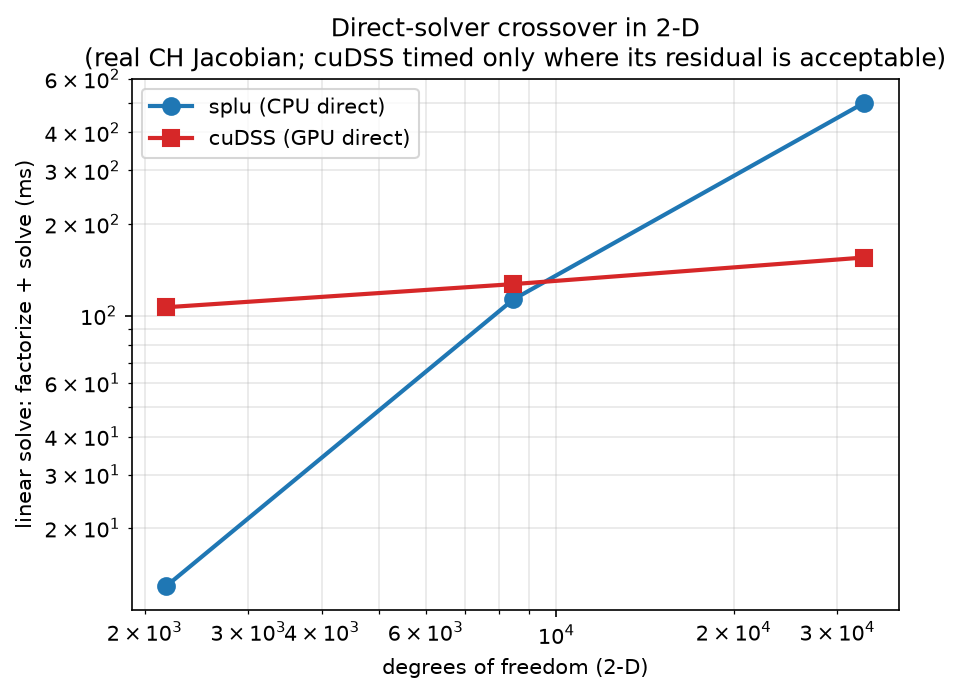
\includegraphics[width=0.62\linewidth]{figures/c4_crossover.png}
  \caption{Direct-solver crossover in 2-D on the real Cahn--Hilliard
    Jacobian: CPU \code{splu} wins at small sizes (GPU overhead dominates),
    GPU cuDSS wins as the problem grows. Timings vary run-to-run; the
    crossover shape does not.}
  \label{fig:c4cross}
\end{figure}

\section{The 3-D wall is memory, not accuracy}

The 3-D numbers take minutes per step to produce, so we cite the
development notes' measured tables. The picture is decisive
(Fig.~\ref{fig:c4cited}) --- and it is about \emph{memory}:
\begin{itemize}[nosep]
  \item cuDSS's factorization fill hits the 48\,GB card at
        $\sim\CfourCudssCeiling$ dofs --- a $>16$\,min factorization that
        never returns. This is a \emph{memory} ceiling; where it fits,
        cuDSS is accurate.
  \item \code{blockch\_dev} beats cuDSS $\CfourBlockchSpeedup\times$ on the
        slab64 solve \emph{and} keeps marching at $\CfourCudssCeiling$
        dofs, where cuDSS ceilings, because it never forms the full LU.
  \item a \emph{block-masked} cuDSS pattern cuts the 3-D fill
        ($17.7\to\CfourMaskedScall$ s/call) --- a strong option below the
        ceiling.
  \item \textbf{AMGX verdict: no.} At production $\Delta t$ the inner
        solves are mass-dominated (well-conditioned), so algebraic
        multigrid has no $O(h^{-1})$ growth to flatten.
  \item matrix-free (and \code{blockch}) push the ceiling to
        $\CfourMatrixfreeDofs$ dofs on a single 48\,GB card.
\end{itemize}

\begin{keybox}
\textbf{A note on preconditioner design.} That the two-factor
\texttt{blockch} preconditioner \emph{exists} is itself a hard-won result:
several \emph{naive} block preconditioners \emph{diverge} on the stiff
Flory--Huggins log potential (documented design-laws in
\file{src/diffsim/solvers/linsolve.py}). That is a statement about
approximate preconditioners --- not about a pivoted direct solve, which is
accurate on the same systems.
\end{keybox}

\begin{figure}[h]\centering
  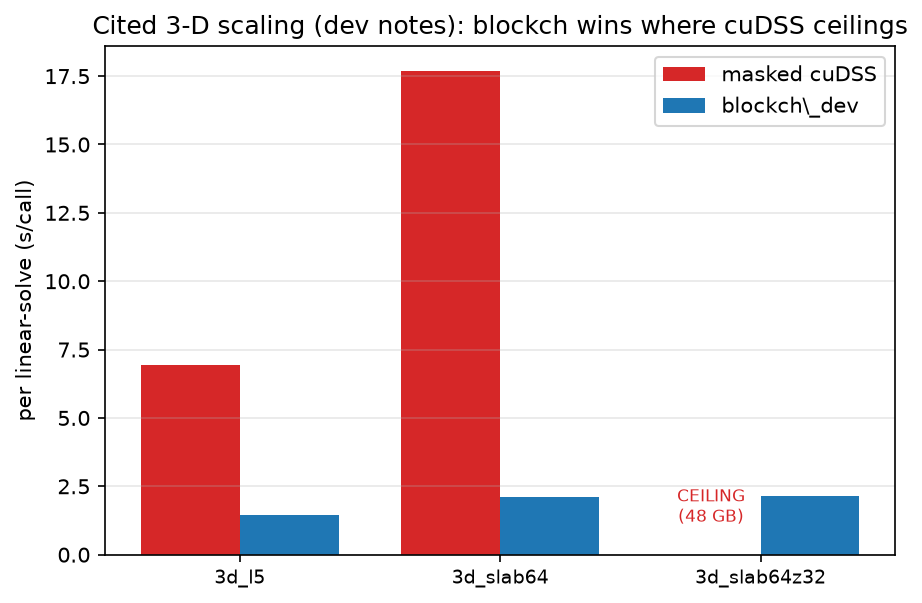
\includegraphics[width=0.72\linewidth]{figures/c4_cited3d.png}
  \caption{Cited 3-D per-solve cost (dev notes): masked cuDSS versus
    \code{blockch\_dev}. blockch is $\CfourBlockchSpeedup\times$ cheaper at
    slab64 and keeps marching at the size where cuDSS's factorization
    ceilings on 48\,GB memory.}
  \label{fig:c4cited}
\end{figure}

\section{Decision support, with a rationale}

Rather than a one-line \code{choose\_solver(dim, dofs)}, the tutorial's
\code{recommend\_solver} weighs dofs, nnz, block structure, precision,
memory, factorization reuse, tolerance, $\Delta t$, and hardware, and
returns a \emph{rationale}, not just a name:
\begin{center}\small
\begin{tabular}{lll}
\toprule
regime & dofs (order) & recommendation \\
\midrule
2-D, small        & $<2\times10^4$   & \code{splu} (pivoted, no GPU overhead) \\
2-D, large        & $<5\times10^5$   & cuDSS (fast, verified accurate) \\
3-D, small        & $<5\times10^5$   & masked cuDSS / \code{blockch\_dev} \\
3-D, large        & up to $\sim1.5\times10^6$ & \code{blockch\_dev} (memory) \\
3-D, extreme      & $>$ int32 / memory & matrix-free (or multi-GPU) \\
\bottomrule
\end{tabular}
\end{center}
Every recommendation carries the caveat to \emph{verify the residual} of a
non-pivoting direct solve, and names \emph{why} (size, fill, memory) so the
choice transfers when the hardware or problem changes.

\section{Code walk-through}

\paragraph{Capturing the real operator (supported API).}
\begin{lstlisting}
st = CahnHilliardStepper(..., capture_system=True)   # no monkeypatch
st.step()
A, b = st.last_system        # the exact saddle a solver would factor
\end{lstlisting}
The benchmark captures the operator through a supported stepper flag ---
not by monkeypatching \code{solve\_linear}. It warms up a few steps so the
residual $b$ is non-trivial (a consistent-$\mu$ step-0 iterate has
$b\approx0$, which makes a relative-residual test degenerate).

\paragraph{Correctness beside speed.}
\begin{lstlisting}
solver_correctness()          # residual + iters of splu / cuDSS / blockch
benchmark_solvers_2d()        # cold+warm, CUDA-synced, median timing
recommend_solver(dofs, dim)   # a rationale, not just a name
\end{lstlisting}
If cuDSS is unavailable, the benchmark degrades gracefully (it skips the
GPU rows and \code{recommend\_solver} falls back to \code{splu}/blockch).

\section{Explore on your own}

\question{Extend the live 2-D sweep to level~8 ($\sim1.3\times10^5$ dofs).
Does cuDSS's lead over \code{splu} keep growing, and does the solve time
scale closer to $O(n)$ or $O(n^{1.5})$? What does the exponent say about
2-D direct fill-in?}

\question{You verified cuDSS is accurate on the 2-D saddle. Construct a
system where a non-pivoting direct solve \emph{should} struggle (hint:
push the FH potential to the regularization cap, or shrink $\Delta t$ so
$\sigma$ is huge) and re-measure the residual. Does the verification still
pass? This is the experiment that separates folklore from measurement.}

\question{The dev note reports \code{blockch\_dev} at $8.4\times$ cuDSS on
the slab64 \emph{solve} but only $2.6\times$ on the \emph{step}. What does
the rest of the step cost, and why does the solver speedup not carry
through one-to-one?}

\question{Using the measured cuDSS ceiling ($\sim\CfourCudssCeiling$ dofs
on 48\,GB), estimate the ceiling on an 80\,GB A100. For a
$96\times96\times48$ film, which solver, and would masked cuDSS change your
answer?}

\question{Add \code{fp32} to \code{recommend\_solver}'s reasoning: halving
the precision halves memory and bandwidth, but the CH condition number may
demand fp64 for the tolerance. Design the experiment (fp32 solve, fp64
residual check) that decides whether fp32 is safe for a given problem.}
